\documentclass[border=10pt]{standalone}

\usepackage{tikz}
\usepackage{tikzsymbols}
\usetikzlibrary{calc,patterns,shapes.geometric}

\def\centerarc[#1](#2)(#3:#4:#5){\draw[#1] ($(#2)+({#5*cos(#3)},{#5*sin(#3)})$) arc (#3:#4:#5);}

\begin{document}
	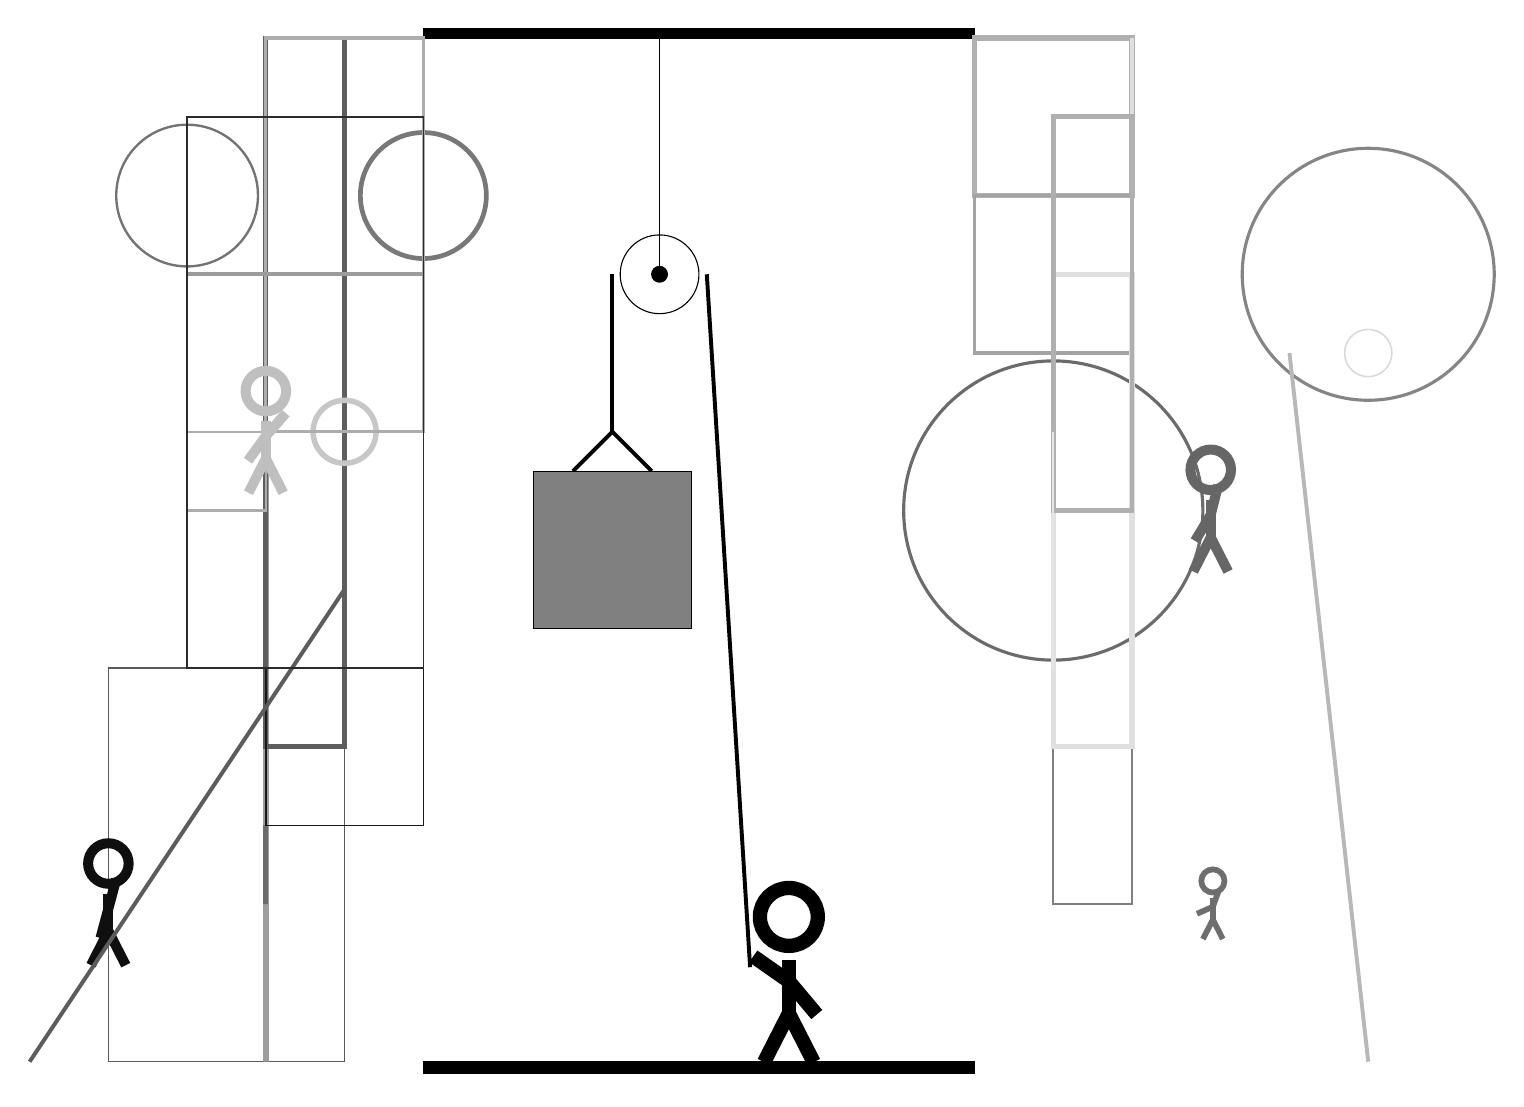
\begin{tikzpicture}
		%%%%% START %%%%%
		
		\draw[fill=black] (-2, 10) rectangle (5, 10.125);
		
		\draw[line width=0.7mm, color=black!31] (7, 8) rectangle (5, 10);
		
		\draw[line width=0.2mm, color=black!65] (-3, 2) rectangle (-6, -3);
		\draw[line width=0.7mm, color=black!38] (-4, -3) rectangle (-4, 5);
		\draw [line width=0.3mm, color=black!55](-5, 8) circle (0.9);
		\draw [line width=0.6mm, color=black!53](-2, 8) circle (0.8);
		\node[line width=0.2mm, color=black!57] at (8, -1) {\Strichmaxerl[4][24][70]};
		\draw[line width=0.3mm, color=black!50] (6, 7) rectangle (7, 9);
		\draw[line width=0.3mm, color=black!40] (-2, 1) rectangle (-2, 1);
		\draw[line width=0.6mm, color=black!58] (-4, -1) rectangle (-4, 0);
		
		\draw[line width=0.6mm, color=black!63] (-3, 10) rectangle (-4, 1);
		
		\draw[line width=0.3mm, color=black!50] (6, -1) rectangle (7, 9);
		\node[line width=0.2mm, color=black!94] at (-6, -1) {\Strichmaxerl[7][75][75]};
		\draw [line width=0.7mm, color=black!22](-3, 5) circle (0.4);
		
		\draw [line width=0.4mm, color=black!58](6, 4) circle (1.9);
		\draw[line width=0.4mm, color=black!32] (-4, 5) rectangle (-2, 10);
		\draw [line width=0.4mm, color=black!48](10, 7) circle (1.6);
		
		\draw[line width=0.4mm, color=black!36] (5, 8) rectangle (7, 6);
		\node[line width=0.4mm, color=black!60] at (8, 4) {\Strichmaxerl[7][59][76]};
		\draw [line width=0.2mm, color=black!15](10, 6) circle (0.3);
		
		\draw[line width=0.2mm, color=black!90] (-2, 0) rectangle (-4, 2);
		\draw[line width=0.7mm, color=black!12] (7, 1) rectangle (6, 7);
		
		\draw[line width=0.5mm, color=black!64](-7, -3) -- (-3, 3);
		\draw[line width=0.6mm, color=black!13] (7, 10) rectangle (7, 5);
		\draw[line width=0.5mm, color=black!39](-2, 7) -- (-5, 7);
		\draw[line width=0.3mm, color=black!32] (-4, 5) rectangle (-5, 4);
		
		\draw[line width=0.6mm, color=black!31] (6, 4) rectangle (7, 9);
		
		\node[line width=0.7mm, color=black!25] at (-4, 5) {\Strichmaxerl[7][54][49]};
		\draw[line width=0.3mm, color=black!10] (6, 2) rectangle (6, 5);
		\draw[line width=0.5mm, color=black!28](10, -3) -- (9, 6);
		\draw[line width=0.2mm, color=black!83] (-2, 2) rectangle (-5, 9);
		
		\draw (1, 7) circle (0.5);
		\draw[fill=black] (1, 7) circle (0.1);
		\draw (1, 10) -- (1, 7);
		
		\draw[line width=0.5mm] (-0.1, 4.5) -- (0.4, 5.0) -- (0.9, 4.5);
		\draw[fill=black!50] (-0.6, 4.5) rectangle (1.4, 2.5);
		
		\draw[line width=0.5mm] (0.4, 7) -- (0.4, 5.0);
		\centerarc[line width=0.5mm](1, 7)(0:180:0.6);
		\draw[line width=0.5mm](1.6, 7) -- (2.15, -1.8);
		
		\node at (2.6, -1.9) {\Strichmaxerl[10][-35][-50]};
		
		\draw[fill=black] (-2, -3) rectangle (5, -3.15);
		
		%%%%% END %%%%%
	\end{tikzpicture}
\end{document}